% !TeX spellcheck = cs_CZ
%{\tikzset{external/prefix={tikz/FYZII/}}
% \tikzset{external/figure name/.add={ch06_}{}}
%---------------------------------------------------------------------------------------------------
% file fey1ch08.tex
%---------------------------------------------------------------------------------------------------
%====================Kapitola: Elektrostatická energie =============================================
\setchaptertoc
\chapter{Elektrostatická energie}\label{fyz:IIchapVI}
  \section{Elektrostatická energie nábojů. Homogenní koule}\label{fyz:IIchapVIsecI}
    Jedním z nejzajímavějších a nejužitečnějších objevů v mechanice byl zákon zachování energie.
    Vzorce pro kinetickou a potenciální energii mechanické soustavy nám pomáhají objevit souvislosti
    mezi stavy soustavy ve dvou různých časech, aniž bychom museli vnikat do podrobností toho, co se
    mezi tím děje. Nyní se chceme zabývat energií elektrostatických soustav. I v nauce o elektřině
    bude princip zachování energie užitečný při objevování mnoha zajímavých věcí.

    Zákon o energii vzájemného působení je v elektrostatice velmi jednoduchý; vlastně jsme ho již
    probírali. Představte si, že máme dva náboje \(q_1\) a \(q_2\) vzdálené od sebe o \(r_{12}\).
    Tato soustava se vyznačuje nějakou energií, neboť na to, aby se oba náboje přivedly do jejich
    současné vzájemné polohy, bylo třeba vynaložit určité množství práce. Práci, která je vykonána
    při přiblížení dvou nábojů z velké vzdálenosti, jsme už počítali. Je rovna
    \begin{equation}\label{fyz:eq868}
      \dfrac{q_1q_2}{4πϵ_0r_{12}}.      
    \end{equation}
    Kromě toho z principu superpozice víme, že v případě mnoha nábojů je celková síla působící na
    každý z nich rovna součtu sil, kterými na něj působí všechny ostatní náboje. Z toho vyplývá, že
    celková energie soustavy více nábojů je rovna součtu členů pocházejících ze vzájemné interakce
    každého páru nábojů. Jsou-li \(q_i\) a \(q_j\) některé dva z těchto nábojů a \(r_{12}\) je
    vzdálenost mezi nimi (\ref{fyz:fig178}), energie tohoto páruje
    \begin{equation}\label{fyz:eq869}
      \dfrac{q_iq_j}{4πϵ_0r_{ij}}.      
    \end{equation}

    \begin{figure}[ht!]  %\ref{fyz:fig178}
      \centering
      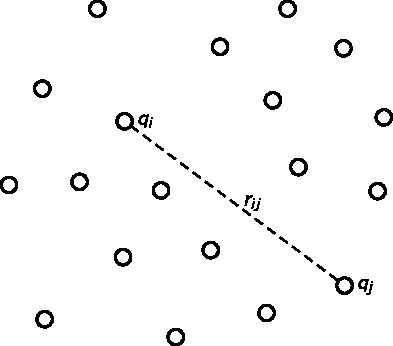
\includegraphics[width=0.6\linewidth]{fyz_fig178.pdf}
      \caption{Elektrostatická energie soustavy částic je rovna součtu elektrostatických energií
              všech párů částic v soustavě (\cite[s.~140]{Feynman02}).}
      \label{fyz:fig178}
    \end{figure}

    Výsledná elektrostatická energie \(W\) je součtem energií všech možných párů nábojů v soustavě:
    \begin{equation}\label{fyz:eq870}
      W=\sum_{\mathclap{\substack{\text{všechny}\\\text{páry}}}}\dfrac{q_iq_j4πϵ_0}{r_{ij}}.
    \end{equation}
    Jde-li o rozdělení nábojů specifikované hustotou náboje \(ρ\), je samozřejmě nutné nahradit sumu
    ve vzorci (\ref{fyz:eq870}) integrálem.

    My se budeme touto energií zabývat ze dvou hledisek. Jedním je \emph{využití} pojmu energie v
    elektrostatických úlohách a druhým jsou různé způsoby výpočtu energie. Někdy je snazší vypočítat
    práci vykonanou v nějakém speciálním případě, než vyčíslit sumu nebo příslušný integrál ve
    vzorci (\ref{fyz:eq870}). Jako příklad vypočtěme energii potřebnou na shromáždění náboje do
    koule s homogenní hustotou náboje. Je rovna práci vykonané při přibližování nábojů z nekonečna.

    Představte si, že kouli vytváříme postupným přikládáním tenkých kulových slupek s
    infinitezimální tloušťkou na sebe. V každém stádiu tohoto procesu bereme malé množství náboje a
    přikládáme jej ve tvaru tenké kulové slupky sahající od \(r\) do \(r + \dd{r}\).


    \begin{figure}[ht!]  %\ref{fyz:fig179}
      \centering
      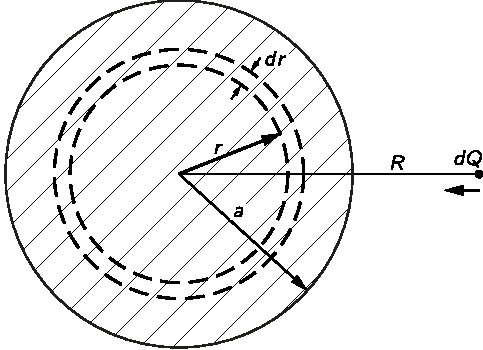
\includegraphics[width=0.6\linewidth]{fyz_fig179.pdf}
      \caption{Energii homogenně nabité koule můžeme počítat tak, že si představíme kouli, jako by
              byla složena ze vzájemně na sebe přiléhajících kulových slupek.
              (\cite[s.~141]{Feynman02}).}
      \label{fyz:fig179}
    \end{figure}

  \section{Energie kondenzátoru. Síly působící na nabité vodiče}\label{fyz:IIchapVIsecII}

    \begin{figure}[ht!]  %\ref{fyz:fig180}
      \centering
      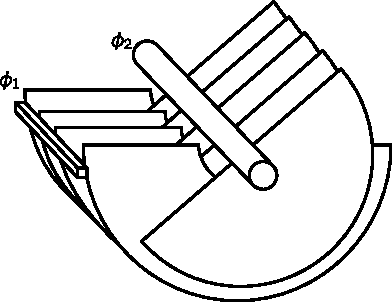
\includegraphics[width=0.6\linewidth]{fyz_fig180.pdf}
      \caption{Jaký moment síly působí na otočný kondenzátor? (\cite[s.~144]{Feynman02}).}
      \label{fyz:fig180}
    \end{figure}
    
    \begin{figure}[ht!]  %\ref{fyz:fig181}
      \centering
      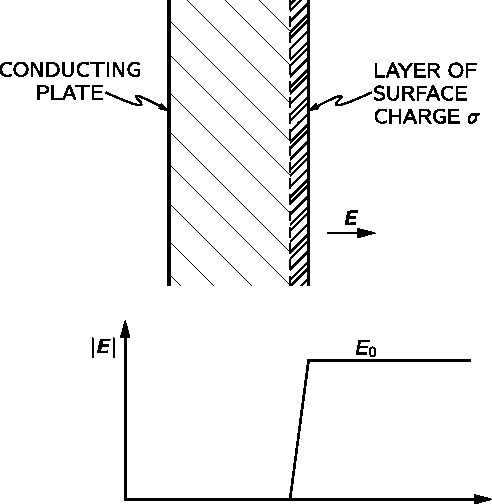
\includegraphics[width=0.6\linewidth]{fyz_fig181.pdf}
      \caption{Intenzita elektrického pole se změní při průchodu vrstvou plošného náboje
              existujícího na povrchu vodiče z nuly na hodnotu \(E_0 =
              \frac{\sigma}{\varepsilon_0}\) (\cite[s.~145]{Feynman02}).}
      \label{fyz:fig181}
    \end{figure}
    
  \section{Elektrostatická energie iontového krystalu}\label{fyz:IIchapVIsecIII}

    \begin{figure}[ht!]  %\ref{fyz:fig182}
      \centering
      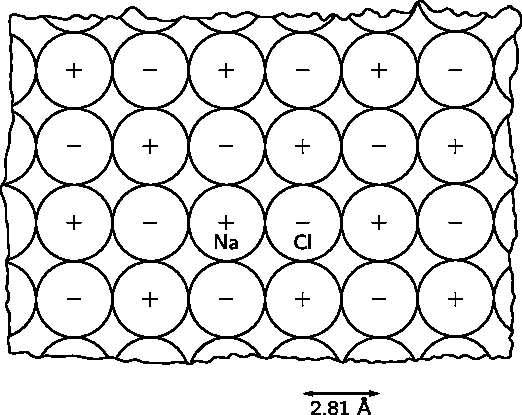
\includegraphics[width=0.6\linewidth]{fyz_fig182.pdf}
      \caption{Řez krystalem kuchyňské soli v atomovém měřítku. Šachovnicové uspořádání iontů \ce{Na} 
              a \ce{Cl} je stené v obou na sebe kolmých řezech krystalem (obr. 1.7 díl I)
              (\cite[s.~146]{Feynman02}).}
      \label{fyz:fig182}
    \end{figure}

  \section{Elektrostatická energie v atomových jádrech}\label{fyz:IIchapVIsecIV}

    \begin{figure}[ht!]  %\ref{fyz:fig183}
      \centering
      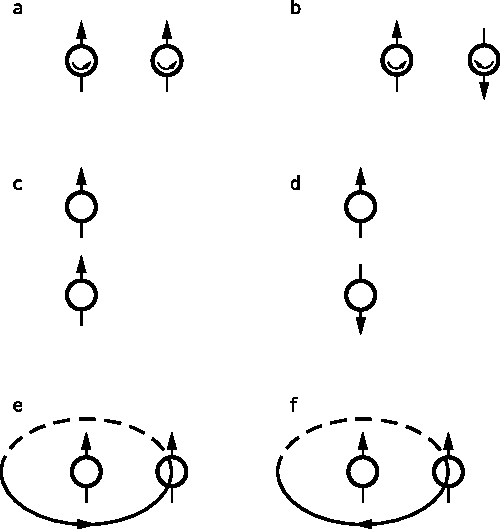
\includegraphics[width=0.6\linewidth]{fyz_fig183.pdf}
      \caption{Síla mezi dvěma protony závisí na všech možných parametrech.
              (\cite[s.~148]{Feynman02}).}
      \label{fyz:fig183}
    \end{figure}

    \begin{figure}[ht!]  %\ref{fyz:fig184}
      \centering
      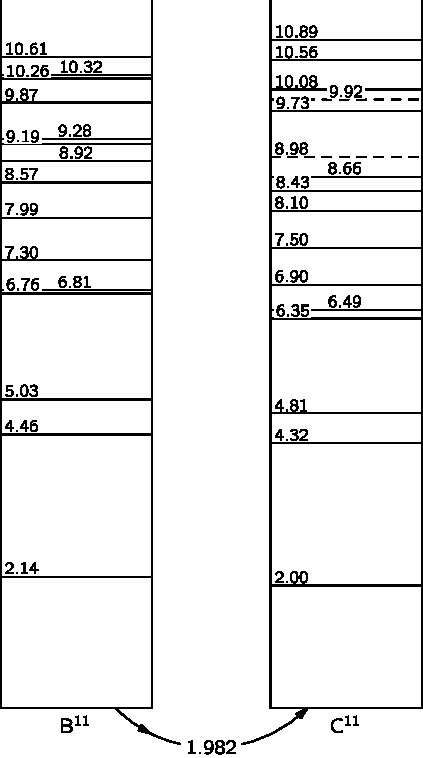
\includegraphics[width=0.6\linewidth]{fyz_fig184.pdf}
      \caption{Energetické hladiny jader \ce{^{11}B} a \ce{^{11}C} (hodnty udané v
              \si{\mega\electronvolt}). Základní stav \ce{^{11}C} leží o
              \SI{1.982}{\mega\electronvolt} výše než základní stav \ce{^{11}B}
              (\cite[s.~149]{Feynman02}).}
      \label{fyz:fig184}
    \end{figure}
    
  \section{Energie v elektrostatickém poli}\label{fyz:IIchapVIsecV}

    \begin{figure}[ht!]  %\ref{fyz:fig185}
      \centering
      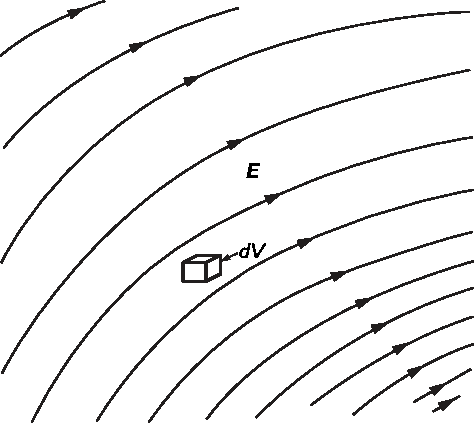
\includegraphics[width=0.6\linewidth]{fyz_fig185.pdf}
      \caption{Každý element objemu \(\dd{V} = \dd{x}\dd{y}\dd{z}\) v elektrickém  poli obsahuje
      energii \(\varepsilon_0/2E^2\dd{V}\) (\cite[s.~154]{Feynman02}).}
      \label{fyz:fig185}
    \end{figure}
    
  \section{Energie bodového náboje}\label{fyz:IIchapVIsecVI}

\todo[inline]{Kapitola fey2ch08 je nedodělaná, obsahuje pouze obrázky}
%} %tikzset
%~~~~~~~~~~~~~~~~~~~~~~~~~~~~~~~~~~~~~~~~~~~~~~~~~~~~~~~~~~~~~~~~~~~~~~~~~~~~~~~~~~~~~~~~~~~~~~~~~~